\section{Support Vector Machines}
\begin{figure}[!h]
    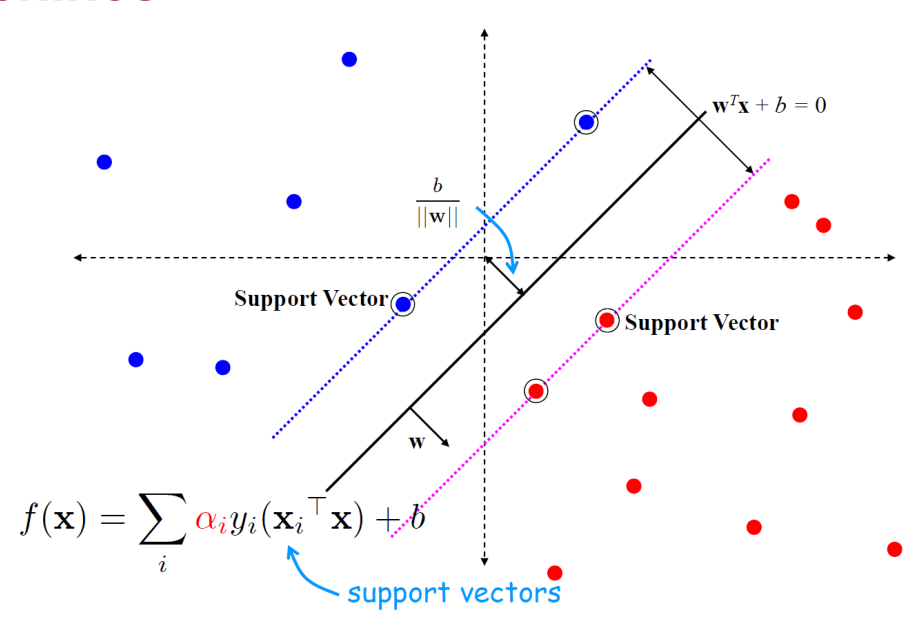
\includegraphics[width = \columnwidth]{figures/08/SVM.png}
\end{figure}
\subsection{Hyperplanes}
Hyperplabes can be modified as:
\[
H_{w,b} = \{\vec{x}|\vec{w}\cdot\vec{x} + b = 0\}
\]
A projection of a point \(x \in \mathbb{R}^p\) onto \(H_w\), i.e., the closest point on \(H_w\) to \(x\) given by:
\[
\pi_w(x) = x-\frac{\langle w,x \rangle + b}{\langle w,w \rangle}\cdot w
\]
A hyperplane \(H_w\) is called separating, if 
\[
\hat{\gamma}_i = y_i \cdot h(x_i) = y_i \cdot (\langle w,x_i \rangle + b) > 0\qquad(i = 1\dots n)
\]
\subsection{maximal margin classifier}
The data is called linear separable if there exists a separating hyperplane.
In general, if there is one, there are many.
We can define our classifier as:
\[
f_{w,b}(x) = \text{sign}(\langle w,x\rangle + b)
\]
Problem: Not invariant of rescaling.
We need some sort of normalization.

We define the geometric margin \(\gamma_i\) of \((w,b)\) with respect to a training sample \((x_i,y_i)\) as:
\[
\gamma_i = y_i \cdot \left(\frac{\langle w,x_i \rangle + b}{||w||}\right) = \frac{\hat{\gamma}_i}{||w||} = y_i d(x_i)
\]
The geometric margin with respect of a training set \(\mathcal{S}\) is smallest of these values in the training set:
\[
\gamma = \min_{i = 1 \dots
n} \gamma_i
\]
The geometric margin is invariant to rescaling of the parameters.
We want to find a classifier that maximizes the geometric margin for linearly seperable dataset.

We will introduce the scaling constraint that the functional margin \(\hat{y}\) of \((w,b)\) with respect to the training set S must be 1: \(\hat{\gamma} = 1\)
\[
\min_{w,b}\left\{\frac{1}{2} ||w||_2^2\right\}
\]
\[
\text{s.t.} \qquad y_i(\langle w,x_i \rangle + b) \ge 1
\]
This is a convex optimization problem that could be solved using a Quadratic Programming (QP) code.
\subsection{Support Vector Classifier SVC}
The hyperplane is only dependent on the vectors closest to it.
The closest vectors are called support vectors after their function.

SVM loss function in dual form:
\[
-\frac{1}{2}\sum_{i = 1}^{n}\sum_{j = 1}^{n}\alpha_i\alpha_j y_i y_j\langle \phi(x_i),\phi(x_j) \rangle + \sum_{i = 1}^{n} \alpha_i
\]

The Representor Theorem states that the solution \(w^*\) of the optimization problem can always be written as a linear combination of the training (or \(\phi\)-transformed training) data:

\[
w^* = \sum_{i = 1}^{N}\alpha_i y_i x_i \qquad w^* = \sum_{i = 1}^{N}\alpha_i y_i \phi(x_i)
\]
\subsubsection{Handling data that is not linearly separable}
\begin{enumerate}
    \item Apply a feature transform \(\phi(x)\)
    \item Introduce slack variables \(\xi\)(tolerate some missclassification)
\end{enumerate}
By increasing the dimensionality of the feature space using mapping \(\phi\), we can find linearly separating hyperplanes.
\subsubsection{Soft margin solution}
\begin{figure}[!h]
    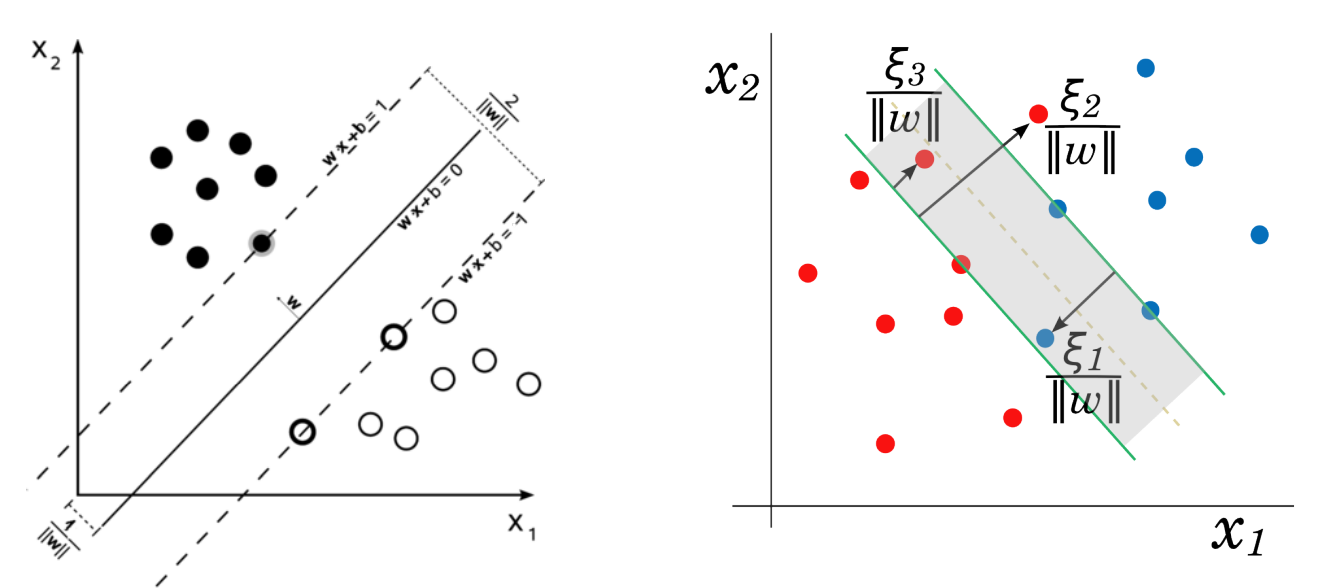
\includegraphics[width = \columnwidth]{figures/08/SoftMargin.png}
\end{figure}
Mathematically, we formulate the trade-off by slack-variables \(\xi_i > 0\).
\[
\min_{w,b}\left\{\frac{1}{2}||w||_2^2 + C\sum_{i}\xi_i\right\}
\]
\[
\text{s.t.} \qquad y_i(\langle w,\phi(x_i) \rangle + 1) \ge 1 - \xi_i
\]
We can fulfill every constraint by choosing \(\xi_i\) large enough.
The larger \(\xi_i\) the larger the objective (that we try minimize).
C is a regulariztion/trade-off parameter:
\begin{itemize}
    \item small C: allow constraints to be easily ignored. Nearly no penalty for misclassification, large margin
    \item large C: makes constraints hard to ignore ! smaller margin, strong penalty for misclassification
    \item C = \(\infty\): recovers a hard margin: all constraints must be fulfilled.
\end{itemize}
\subsubsection*{Non separable case example}
\begin{figure}[!h]
    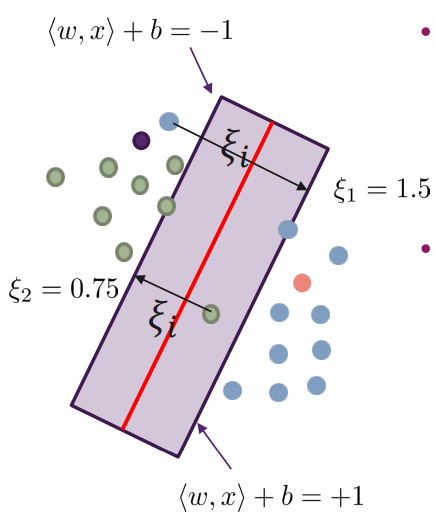
\includegraphics[width = 0.3\columnwidth]{figures/08/SoftMarginExample.png}
\end{figure}
\[
y_1(\langle w,x_1 \rangle + b) \ge 1 - 1.5 = 0.5
\]
\[
y_2(\langle w,x_2 \rangle + b) \ge 1 - 0.75 = 0.25
\]
\[
\sum_{i} \xi_i = 1.5 + 0.75 = 2.25
\]
\subsubsection*{Influence of the regulariztion parameter \(C\)}
\begin{figure}[!h]
    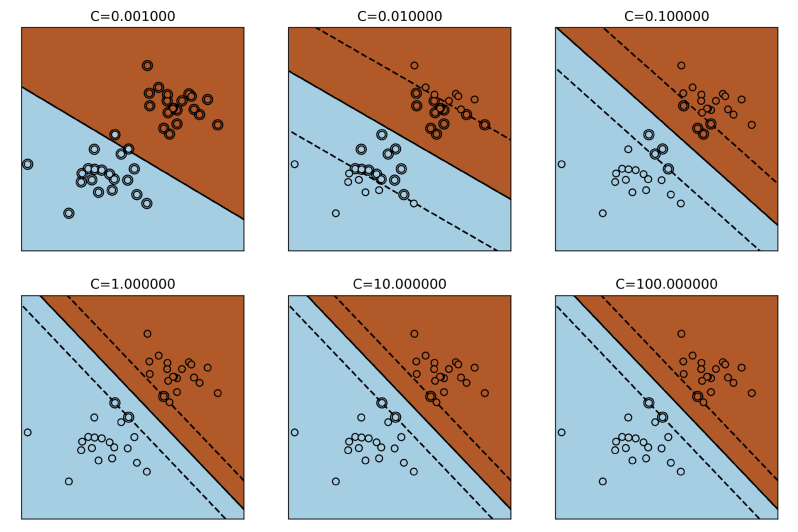
\includegraphics[width = \columnwidth]{figures/08/CExamples.png}
\end{figure}
\subsection{Support Vector Machine SVM}
\subsubsection{The Kernel Trick}
Because of the Kernel Trick, a fir on kernel-transformed data can be done implicitly - that is, without ever building the full \(N\)-dimensional representation of the kernel projection.
This kernel trick is built into the SVM, and is one of the reasons the method is so powerful.
\subsubsection{Kernel Functions}
Note that \(\phi(x)\) only occures in pairs: \(\langle \phi(x_i),\phi(x_j) \rangle = \phi^T(x_i)\cdot \phi(x_j)\)

The complexity of learning depends on \(N\)(Data points), typically it is \(O(N^3)\), not on D(Dimensions of Kernel space)
\[
f(x) = \sum_{i =1}^{N}\alpha_i y_i K(x_i,x) + b
\]
\(\alpha\): weights, might be zero

\(x_i\): Support Vector(only few)

Kernel Function:
\[
K_{ij} = K(x_i,x_j) = \langle \phi(x_i),\phi(x_j) \rangle = \langle z_i, z_j \rangle
\]
\(K_{ij}\) is calculated fast, \(z_i = \phi(x_i)\) is hard to calculate.
Leads to the same optimization problem as the original dual optimization problem.
\subsubsection{Primal Form of the SVM}
\[
\min_{\mathbf{w},b,\mathbf{\xi}}\frac{1}{2}||w||_2^2 + C \sum_{i = 1}^{n} \xi_i
\]
\[
y_i(\mathbf{w}\cdot x_i + b) \ge 1 - \xi_i, \quad \forall i = 1,2,\dots,n
\]
\[
\xi_i \ge 0, \quad \forall i = 1,2,\cdot,n
\]
The second term,\(C\sum \xi_i\), incorporates the slack variable \(\xi_i\) and the regularization parameter \(C\).
\(C\) is a hyperparameter that controls the trade-off between maximizing the margin and minimizing the slack variables.
A larger \(C\) encourages a narrower margin but penalizes misclassifications more severly.
\subsubsection{Kernel Trick - Summary}
\begin{itemize}
    \item Classifiers can be learnt for high dimensional feature spaces, without actually having to map the points into high dimensional space
    \item Data may be linear separable in the high dimensional space, but not linearly separable in the original feature space
    \item Kernels can be used for an SVM because of the scalar product in the dual form, but can also be used elsewhere - they are not tied to the SVM formalism
    \item Kernels apply also to objects that are not vectors, e.g. to objects like histograms.
\end{itemize}

